\documentclass[tikz]{standalone}
\usepackage{tikz}
\usepackage{fourier}
\usepackage{physics}
\usetikzlibrary{shapes.geometric}
\usetikzlibrary{calc}

\begin{document}
\begin{tikzpicture}
    % Spherical harmonic plots
    \node[inner sep=0] at (0, 0) {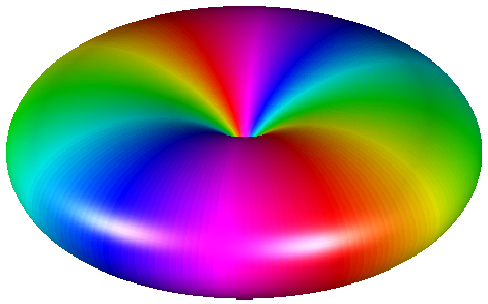
\includegraphics{gfx/FM-2-spherical.pdf}};
    \node[inner sep=0] at (8, 0) {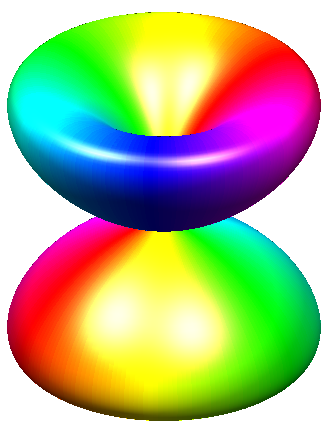
\includegraphics{gfx/FM-1-spherical.pdf}};
    \node[inner sep=0] at (14, 0) {
\includegraphics{gfx/UN-spherical.pdf}};
    \node[inner sep=0] at (21, 0) {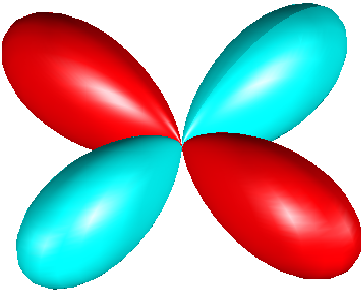
\includegraphics[scale=1.2]{gfx/BN-spherical.pdf}};
    \node[inner sep=0] at (29, 0)
        {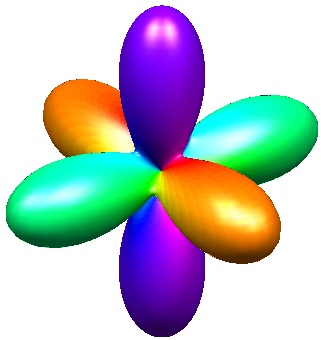
\includegraphics[scale=1.2]{gfx/C1-spherical.pdf}};
        
    % Colour bar
    \node[rotate=90] at (-5, 0) {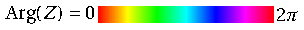
\includegraphics[scale=1.8]{gfx/compiled_hsv.pdf}};
    
    % FM lines
    \draw[->, dashed, line width=2] (0, 0.2) -- (0, 3);
    \draw[->, dashed, line width=2] (8, 1.25) -- (8, 4);

    % Nematic lines
    \draw[-, line width=2] (14, 4.1) -- (14, 5) node[above] {\Huge \(\hat{\vb{d}}\)};
    \draw[->, line width=2] (15.15, 0.) -- (16, 0.) node[right] {\Huge \(C_2\)};
    
    % BN Lines
    \draw[->, line width=2] (21, 0.1) -- (21, 3) node[above] {\Huge \(C_4\)};
    \draw[->, line width=2] (22.5, 0.1) -- (24.5, 0.1) node[right] {\Huge \(C_2'\)};
    \draw[->, line width=2] (24.1, 2.7) -- (24.7, 3.3) node[above] {\Huge \(C_2\)};

    % Cyclic lines
    \draw[->, line width=2] (29, 3.25) -- (29, 4) node[above] {\Huge \(C_2\)};
    \draw[->, line width=2] (31.2, -1.3) -- (32, -1.7) node[below] {\Huge \(C_2\)};
    \draw[->, line width=2] (32.1, 1.2) -- (32.7, 1.45) node[above] {\Huge \(C_2\)};
    \draw[->, line width=2] (29.4, 0.3) -- (31, 2) node[above] {\Huge \(C_3\)};

    % Labels
    \node at (0, -5) {\Huge (a)};
    \node at (8, -5) {\Huge (b)};
    \node at (14, -5) {\Huge (c)};
    \node at (21, -5) {\Huge (d)};
    \node at (29, -5) {\Huge (e)};

    % Axis orientation
    \draw[->, line width=2] (-3.5, -4) -- (-3.5, -3) node[above] {\LARGE \(z\)};
    \draw[->, line width=2] (-3.5, -4) -- (-2.5, -4) node[right] {\LARGE \(x\)};
    \draw[->, line width=2] (-3.5, -4) -- (-3, -3.5) node[right] {\LARGE \(y\)};
\end{tikzpicture}
\end{document}
